\documentclass{article}

\usepackage{graphicx}

\setlength{\parskip}{\medskipamount}

\title{Advanced Object Oriented Programming and Design\\
\medskip
\large Theoretical Homework 2}
\author{Abraham Murciano and Daniel Klein}

\begin{document}

\maketitle

\section*{Question A}

Below is a UML class diagram which describes the relationships between different entities for a hospital, according to the specifications given in the question paper.

\begin{figure}[htbp]
	\centering
	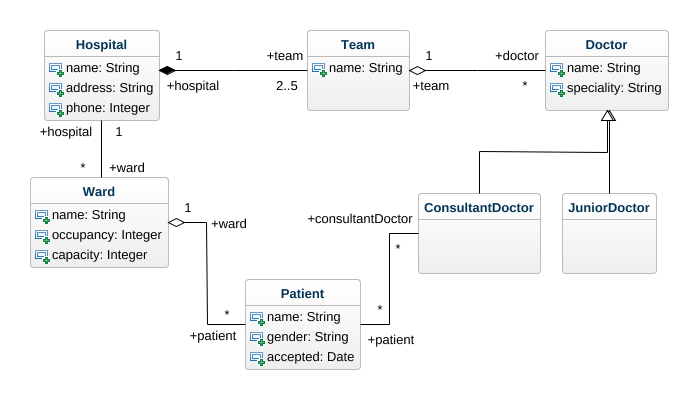
\includegraphics[width=\textwidth]{uml.png}
\end{figure}

\section*{Question B}

The relationship between Hospital and Team is a composition, because there is ownership, meaning a team can belong to at most one hospital, and there is also existence dependance, meaning if a hospital is deleted, so are its teams.

\section*{Question C}

The relationship between Team and Doctor is an aggregation, since there is ownership, meaning a doctor can belong to at most one team at any given time, however there is no existence dependance, since a team can be deleted without its doctors.

\section*{Question D}

The relationship between Doctor and ConsultantDoctor is one of inheritance, since a consultant doctor is a type of doctor.

\section*{Question E}

The relationship between Doctor and JuniorDoctor is one of inheritance, since a junior doctor is a type of doctor.

\section*{Question F}

There is no direct relation between Team and ConsultantDoctor. However, since ConsultantDoctor extends the class Doctor, it inherits the aggregation relation described in question C.

\section*{Question G}

The relationship between Hospital and Ward is a bidirectional association, since we are told that a ward also has a pointer to its hospital. A hospital may have many wards, but obviously a ward can be part of only one hospital.

\section*{Question H}

The relationship between Ward and Patient is an aggregation, since there is ownership, because a patient cannot be in two wards simultaneously. However there is no existence dependance.

\section*{Question I}

There is no direct relation between Team and Patient.

\section*{Question J}

There is no direct relation between Doctor and Patient, since only the sub-type ConsultantDoctor can treat patients.

\section*{Question K}

The relationship between ConsultantDoctor and Patient is a many to many bidirectional association. This is because a consultant doctor can treat many patients and a patient can be treated by any number of consultant doctors.

\end{document}